\documentclass[a4paper, 12pt]{article}

\usepackage{fontspec}
\usepackage{polyglossia}
\defaultfontfeatures{Ligatures=TeX}
\setdefaultlanguage{russian}
\setotherlanguage{english}
\setmainfont{Times New Roman}
\newfontfamily{\latinfont}{Times New Roman}
\newfontfamily{\cyrillicfont}{Times New Roman}
\newfontfamily{\cyrillicfonttt}{Courier New}

\usepackage{geometry}
\usepackage{amsmath}
\usepackage{amssymb}
\usepackage{amsfonts}
\usepackage{graphicx}
\usepackage{float}
\usepackage{wrapfig}
\usepackage{subcaption}
%\usepackage[caption=false]{subfig}
\geometry{right=20mm}
\geometry{left=20mm}
\geometry{top=20mm}
\geometry{bottom=20mm}

\usepackage{indentfirst}
\usepackage[outputdir=auxiliary]{minted}

\graphicspath{{../img/}}
\DeclareMathOperator{\R}{\mathbb{R}}
\DeclareMathOperator{\C}{\mathbb{C}}
\renewcommand{\Re}{\mathrm{Re}}
\renewcommand{\Im}{\mathrm{Im}}


\begin{document}
    \begin{titlepage}
    \begin{center}
        \textit{МИНИСТЕРСТВО ОБРАЗОВАНИЯ И НАУКИ\\
        РОССИЙСКОЙ ФЕДЕРАЦИИ}
        \vspace{1ex}

        федеральное государственное бюджетное образовательное учреждение\\
        высшего профессионального образования
        \vspace{1ex}

        \textbf{САНКТ-ПЕТЕРБУРГСКИЙ НАЦИОНАЛЬНЫЙ ИССЛЕДОВАТЕЛЬСКИЙ УНИВЕРСИТЕТ ИТМО}
        \vspace{13ex}

        Лабораторная работа №3\\
        <<Динамика нелинейных систем>>\\
        по дисциплине <<Моделирование технических систем>>\\
        \vspace{1em}
        Вариант 3\\
    \end{center}
    \vspace{14em}
    \begin{flushright}
        \noindent
        Выполнили:\\
        студенты гр. R4133c\\
        Борисов М. В.\\
        Симонов П.\\
        Мацуганов А. И.\\
        \vspace{1em}
        Преподаватель:\\
        Семенов Д. М.
    \end{flushright}
    \vfill
    \begin{center}
        \large{Санкт-Петербург}\\
        2021 г.\\
    \end{center}
\end{titlepage}

    \setcounter{page}{2}
    \setlength{\parindent}{0pt}

    \section*{Задание 1}
    Дана нелинейная система.
    \begin{equation*}
        \left\{
        \begin{aligned}
            \dot{x} &= -3x + y\\
            \dot{y} &= x - 4y - \arctan{2y}
        \end{aligned}
        \right.
    \end{equation*}

    \begin{enumerate}
        \item Найти её положения равновесия
        \item Линеаризовать систему около одного из положений равновесия, исследовать на устойчивость
        \item Доказать устойчивость исходной системы с помощью метода функций Ляпунова
        \item Построить графики исходной и линеаризованной систем
    \end{enumerate}

    \subsection*{Решение}
    \subsubsection*{Найдём положение равновесия}
    \begin{equation*}
        \left\{
        \begin{aligned}
            &-3x_1 + x_2 = 0 \\
            &x_1 - 4x_2 - \arctan{2x_2} = 0
        \end{aligned}
        \right.
    \end{equation*}
    \begin{equation*}
        \left\{
        \begin{aligned}
            &x_2 = 3x_1 \\
            &11x_1 = -\arctan{6x_1}
        \end{aligned}
        \right.
    \end{equation*}

    \[x^* = (0,\,0)\]

    \subsubsection*{Исследуем на устойчивость около положения равновесия}
    \begin{equation*}
        A(x) =
        \begin{bmatrix}
            -3& 1\\
            1& -\dfrac{6 + 16x^2}{1 + 4x^2}
        \end{bmatrix}
    \end{equation*}

    \begin{equation*}
        A(x^*) =
        \begin{bmatrix}
            -3& 1\\
            1& -6
        \end{bmatrix}
    \end{equation*}

    Собственные числа матрицы $A(x^*)$

    \begin{equation*}
        \begin{aligned}
            \lambda_1 &= -6.30 \\
            \lambda_2 &= -2.70\\
        \end{aligned}
    \end{equation*}

    Оба числа действительные и отрицательные, значит система устойчива и имеет положение равновесия типа "узел".

    \begin{figure}[H]
        \centering
        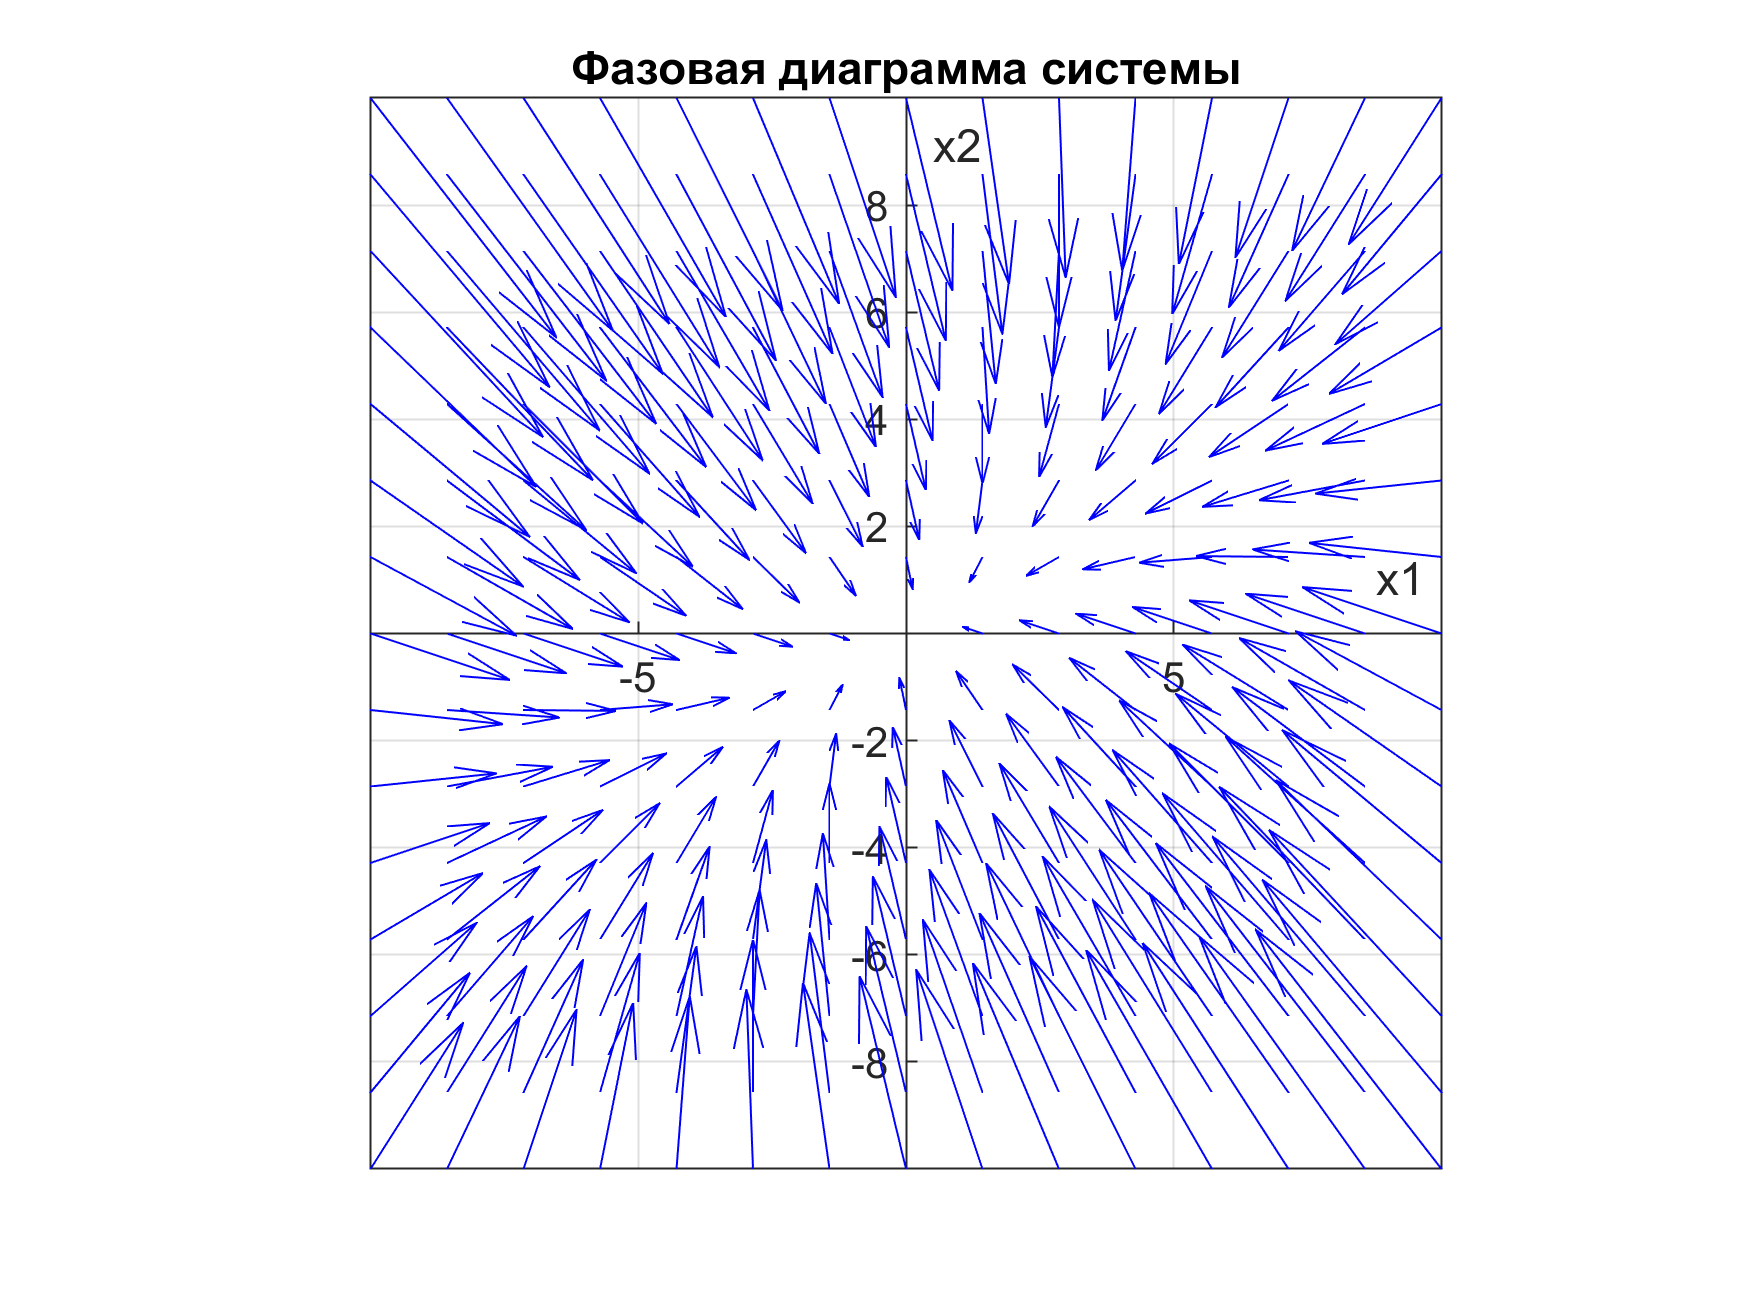
\includegraphics[width=0.7\textwidth]{phase.png}
    \end{figure}

    \subsubsection*{Метод функций Ляпунова}
    \[V(x) = x_1^2 + x_2^2\]
    \[\dot{V}(x) = 4x_1 x_2 - 2x_2\arctan{2x_2} - 6x_1^2 - 8x_2^2\]
    Чтобы доказать $\dot{V}(x) < 0\, \forall x \in X \textbackslash\{0\}$ достаточно показать, что
    \[6x_1^2 + 8x_2^2 > 4x_1 x_2\]
    Член с $\arctan$ можно опустить, т.к. если выражение слева больше без него, то с ним будет ещё больше.
    Приведя неравенство к виду \[3t + \dfrac{4}{t} = 2,\,\mbox{где}\,t = \dfrac{x_1}{x_2}\] получим, что данное уравнение не
    имеет действительных корней и всегда положительно.

    Таким образом $\dot{V}(x) < 0\, \forall x \in X \textbackslash\{0\}$, поэтому исходная система является
    ассимптотически устойчивой.

    \subsubsection*{Графики систем}

    \begin{figure}[H]
        \centering
        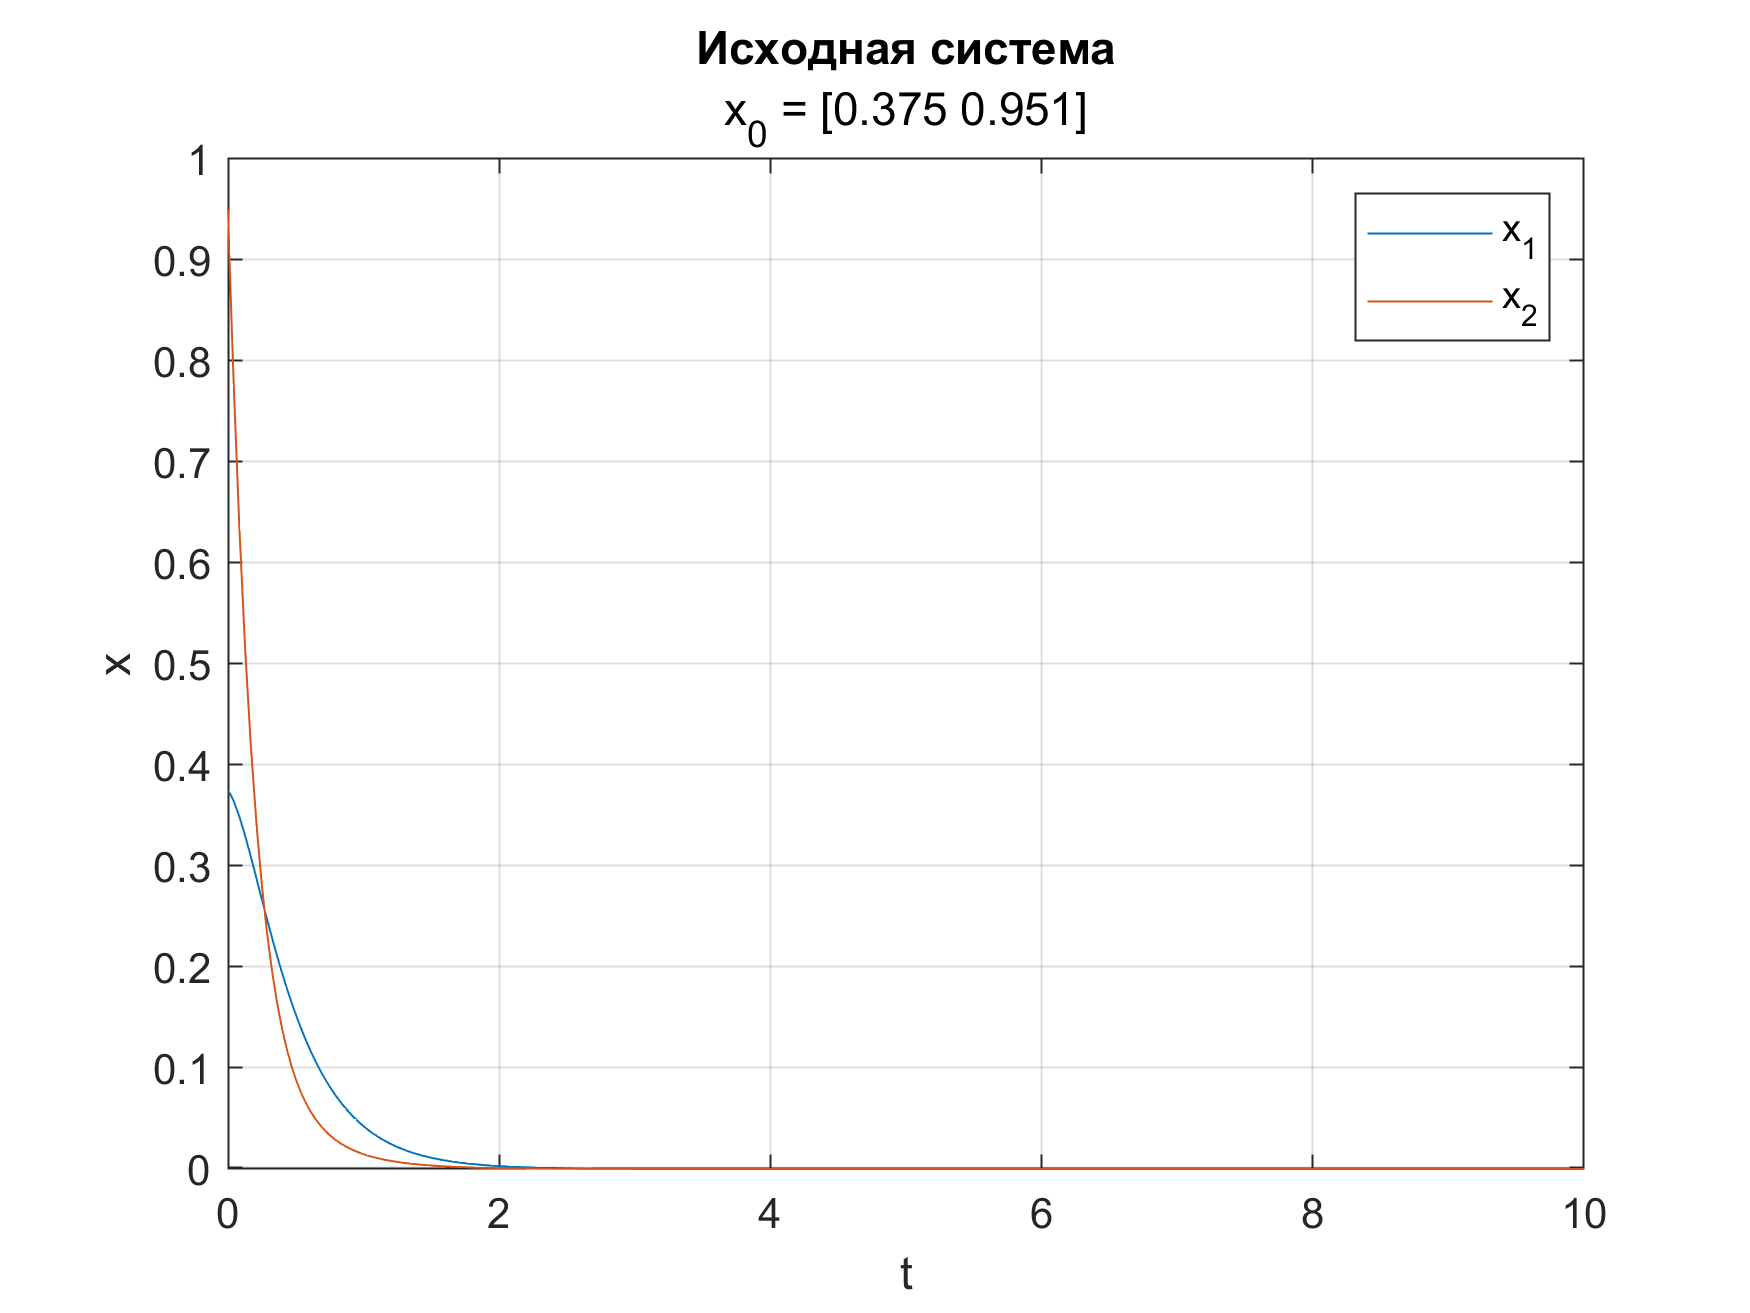
\includegraphics[width=0.7\textwidth]{initial.png}
    \end{figure}

    \begin{figure}[H]
        \centering
        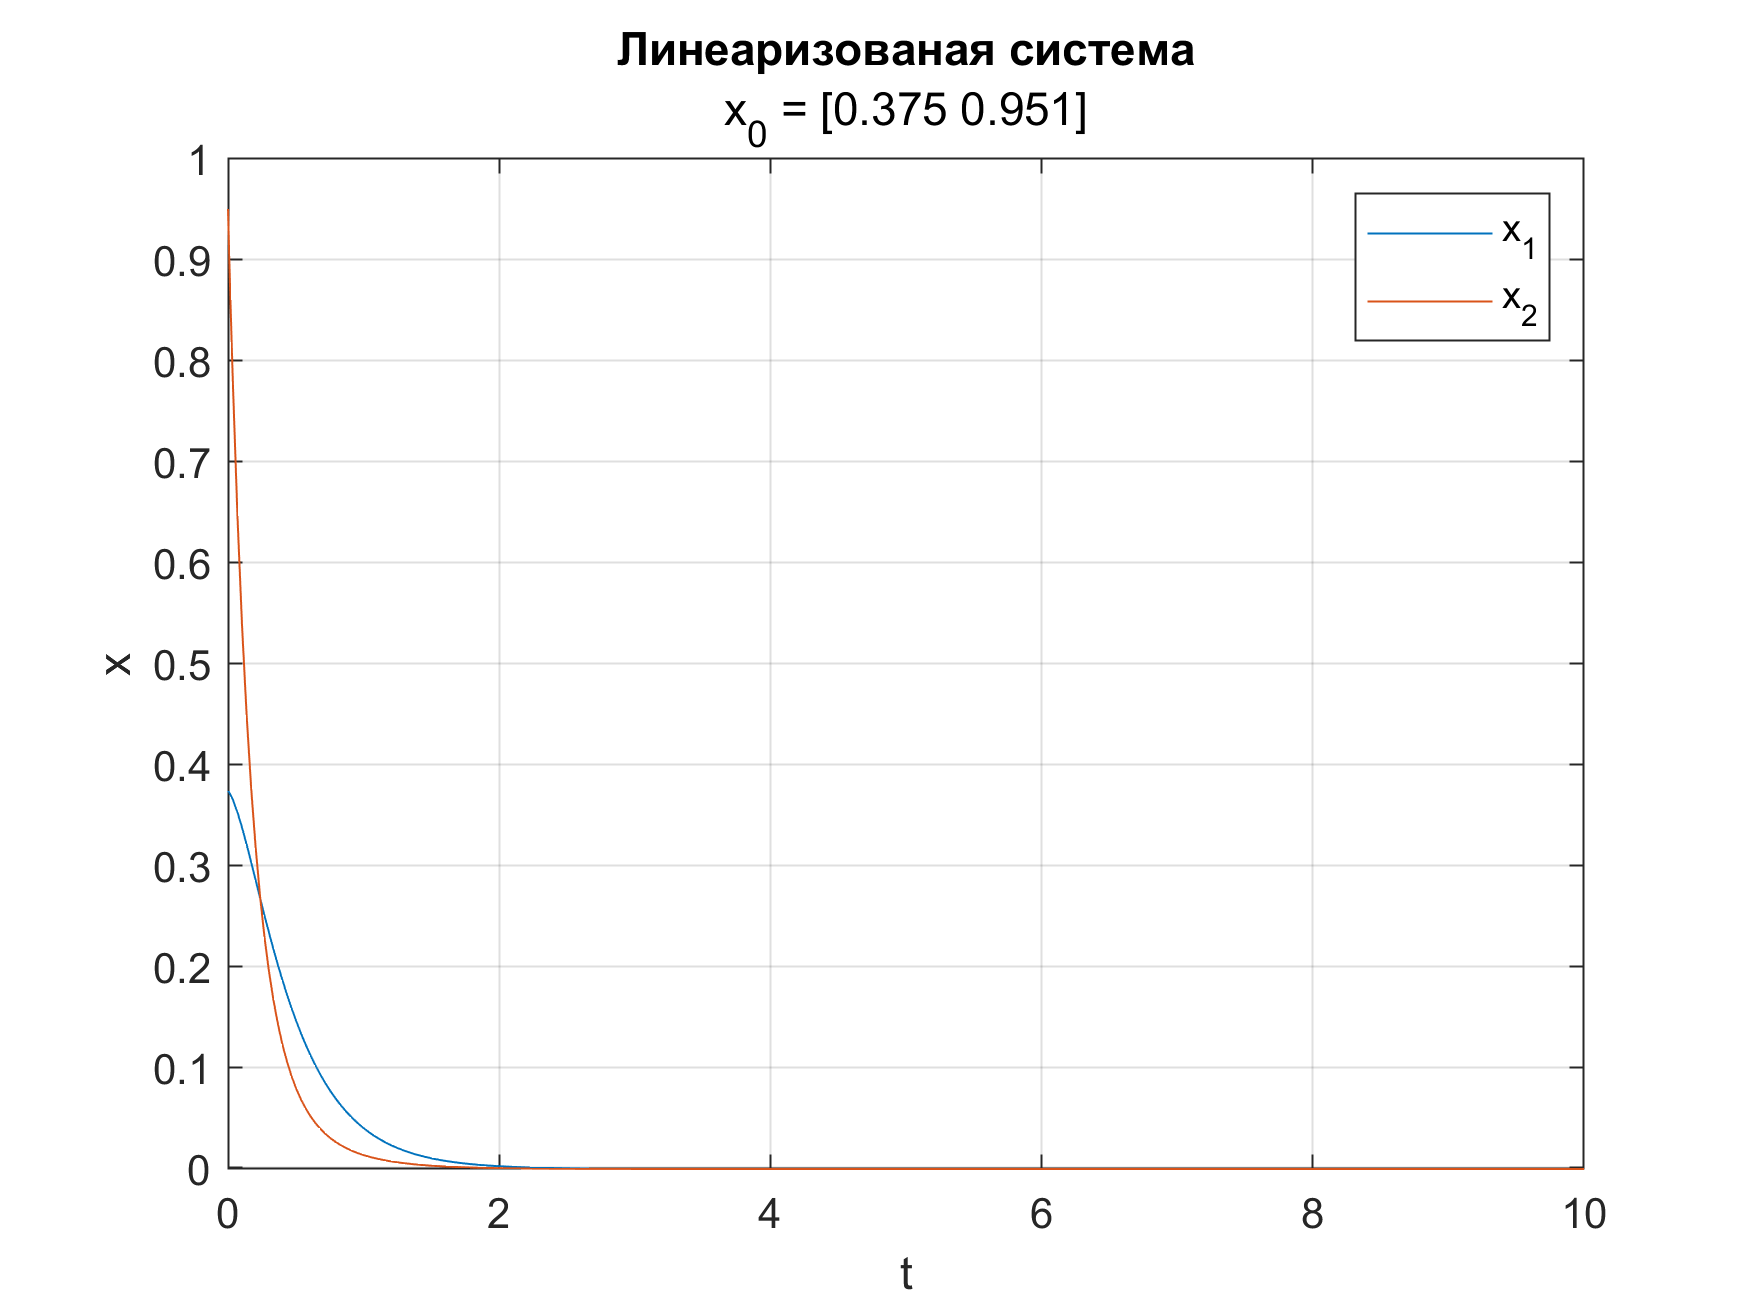
\includegraphics[width=0.7\textwidth]{linearized.png}
    \end{figure}

\end{document}
